\documentclass{article}

\usepackage{ctex}
\usepackage{tikz}
\usetikzlibrary{graphs}

\begin{document}
    % 向量
    \begin{tikzpicture}
        \draw [color=blue!50, ->] 
            (0, 0)
            node [left] {$A$} 
            --
            node [color=red!70, pos=0.5,above, sloped]{Hello}
            (3, 3)
            node [right] {$B$};    
    \end{tikzpicture}

    % 圆,椭圆,矩形,贝塞尔曲线, 扇形
    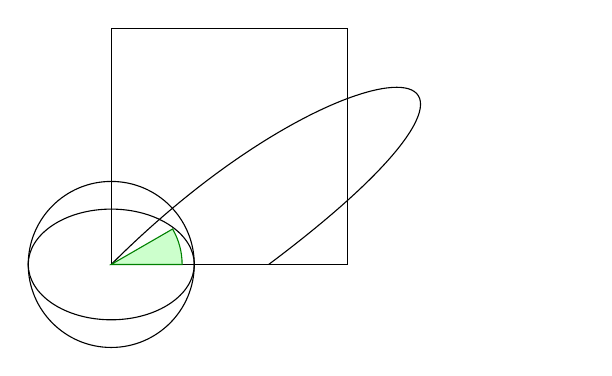
\begin{tikzpicture}
        \draw (0, 0) circle (30pt);
        % 一个起点为(0,0),终点为(2,0)的贝塞尔曲线
        \draw (0, 0 ) ..controls (3, 3) and (6, 3) .. (2, 0);
        % 椭圆
        \draw (0, 0) ellipse (30pt and 20pt);
        \draw (0, 0) rectangle (3, 3);
        % 扇形
        \filldraw [fill=green!20!white, draw=green!50!black]
            (0, 0) -- (9mm, 0mm) arc (0:30:9mm) --cycle;
    \end{tikzpicture}

    % 属性预定义 与 循环
    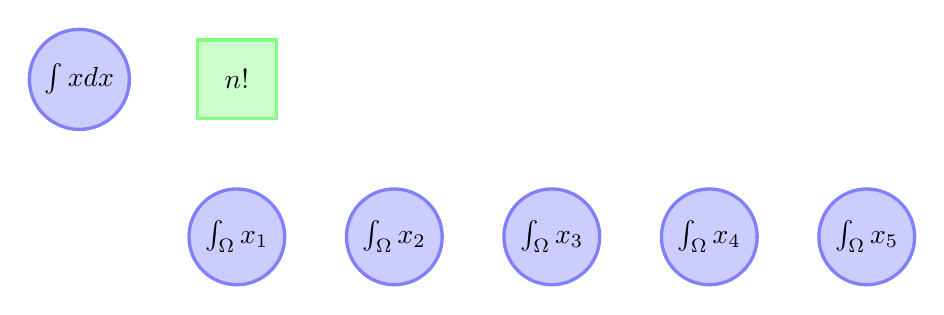
\begin{tikzpicture}
        [   
            L1Node/.style=
            {circle, draw=blue!50,fill=blue!20,
            very thick, minimum size=10mm},
            L2Node/.style=
            {rectangle, draw=green!50, fill=green!20,
            very thick, minimum size=10mm}
        ]
            \node[L1Node] (n1) at (0,0){$\int x dx$};
            \node[L2Node] (n2) at (2,0){$n!$};

            \foreach \x in {1, ..., 5}
                \node[L1Node] (w1_\x) at (2*\x, -2)
                    {$\int_\Omega x_\x$};
    \end{tikzpicture}

    % node树
    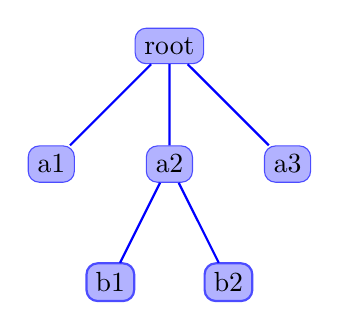
\begin{tikzpicture}
        [
            every node/.style={
                fill=blue!30,draw=blue!70,rounded corners
            },
            edge from parent/.style={blue, thick, draw}
        ]
        \node {root}
            child {node {a1}}
            child {node {a2}
                child {node {b1}}
                child {node {b2}}
            }
            child {node {a3}};
    \end{tikzpicture}

    % 绘制函数图像
    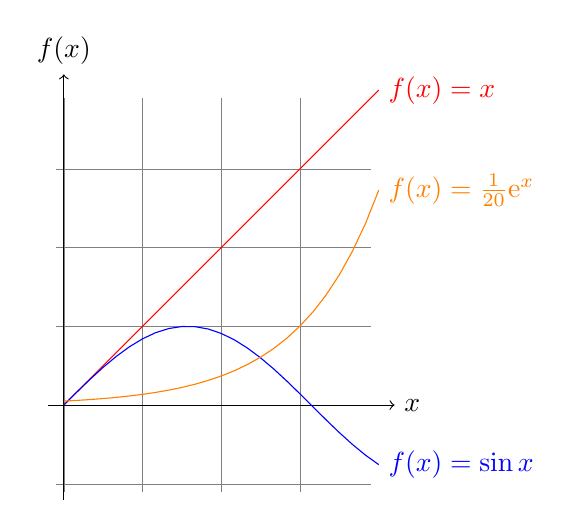
\begin{tikzpicture}
        [domain=0:4]
        \draw[very thin, color=gray] (-0.1, -1.1)grid(3.9, 3.9);
        \draw[->](-0.2, 0) -- (4.2, 0) node[right]{$x$};
        \draw[->](0,-1.2) --(0, 4.2) node[above] {$f(x)$};
        \draw[red] plot(\x, \x) node [right] {$f(x)=x$};
        % \x r 表示弧度
        \draw[blue] plot(\x, {sin(\x r)}) 
            node[right]{$f(x)=\sin x$};
        \draw[orange]plot(\x, {0.05*exp(\x)})
            node[right]{$f(x)=\frac{1}{20} \mathrm e^x$};
    \end{tikzpicture}

    % 图(graphs)的支持
    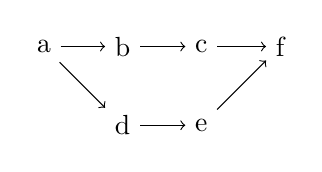
\begin{tikzpicture}
        \graph {
            a -> {
                b -> c,
                d -> e
            } -> f
        };
    \end{tikzpicture}
    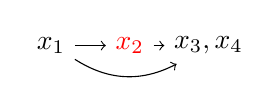
\begin{tikzpicture}
        \graph {
            "$x_1$" -> "$x_2$"[red] -> "$x_3, x_4$";
            "$x_1$" -> [bend right] "$x_3, x_4$";
        };
    \end{tikzpicture}

    
\end{document}